\documentclass{article}
\usepackage{graphicx} % Required for inserting images



\usepackage{amsmath, amsfonts, physics, siunitx, tikz, pgfplots, modiagram, chemfig, mhchem}
\pgfplotsset{compat=1.18}


\title{Radioactive Decay}


\author{Logan Kuhn}
\date{August 2025}

\begin{document}

\maketitle

\section*{Calculating $\tau$}

\begin{gather*}
    \frac{dN}{N}=-\frac{1}{\tau}dt \\
    \int_{N_0}^N\frac{1}{N}dN=-\frac{1}{\tau}\int_{t_0}^t dt \\
    \ln(N)-\ln(N_0)=-\frac{t}{\tau} \\
    \ln\left(\frac{N}{N_0}\right)=-\frac{t}{\tau} \\
    \ln\left(\frac{1}{2}\right)=-\frac{t}{\tau} \\
    T_{1/2}=-\tau*\ln\left(\frac{1}{2}\right) \\
    \tau=-\frac{T_{1/2}}{\ln\left(\frac{1}{2}\right)} \\
    \tau = -\frac{5700}{\ln\left(\frac{1}{2}\right)} \\
    \tau = 8223
\end{gather*}

Therefore the analytic solution is:

$$N(t)=N_0e^{-\frac{t}{8223}}$$

Below can be seen the different step sizes, made with "make carbon WIDTH=[width]" in increasing order of step size (10, 100, 100).

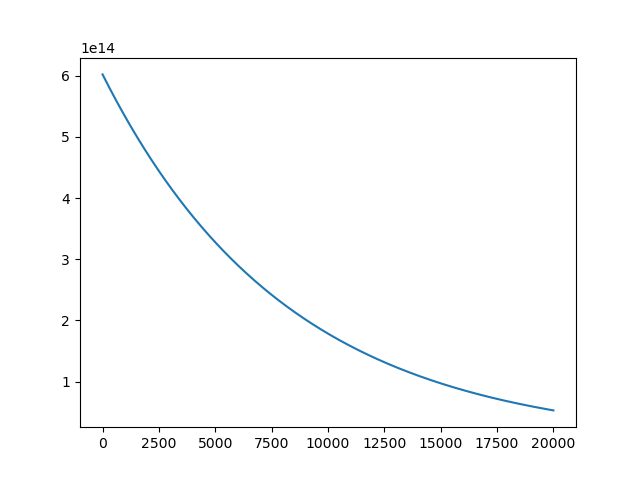
\includegraphics[width=.5\textwidth]{carbonWidth10.png}

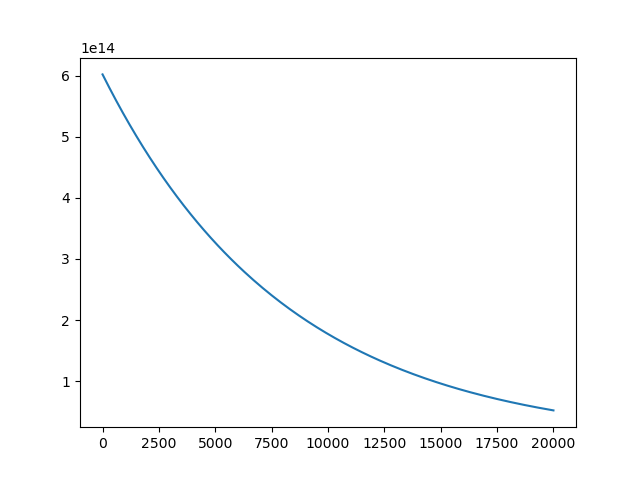
\includegraphics[width=.5\textwidth]{carbonWidth100.png}

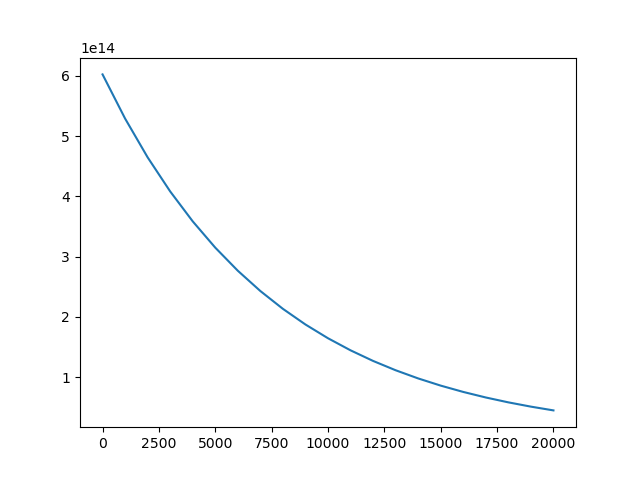
\includegraphics[width=.5\textwidth]{carbonWidth1000.png}

\section*{Golf.py}

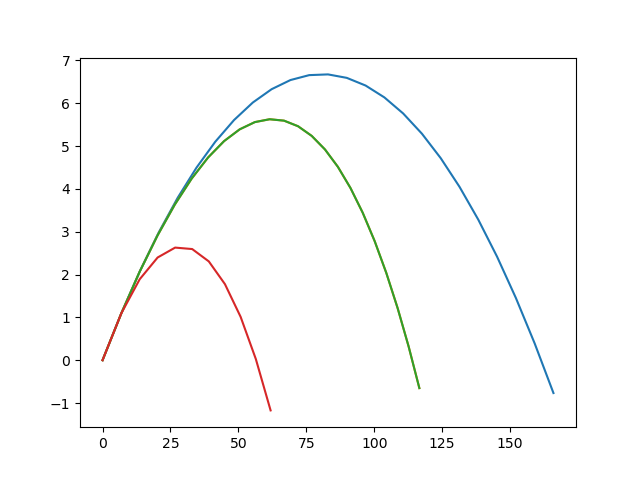
\includegraphics[width=.5\textwidth]{golfPlotTheta9.0.png}
Made with command "make golf THETA=9"


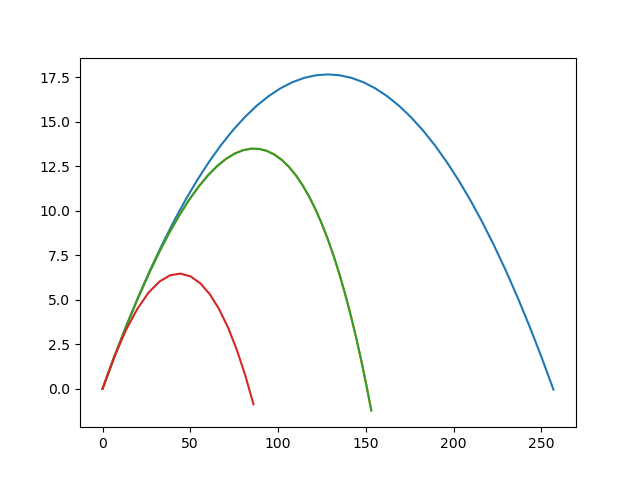
\includegraphics[width=.5\textwidth]{golfPlotTheta15.0.png}
Made with command "make golf THETA=15"

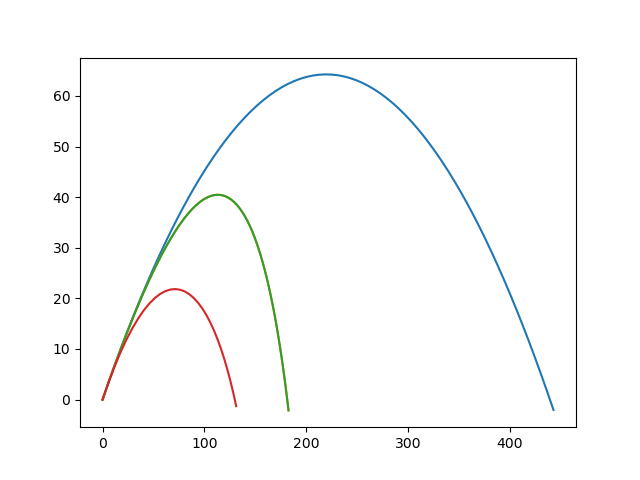
\includegraphics[width=.5\textwidth]{golfPlotTheta30.0.png}
Made with command "make golf THETA=30"


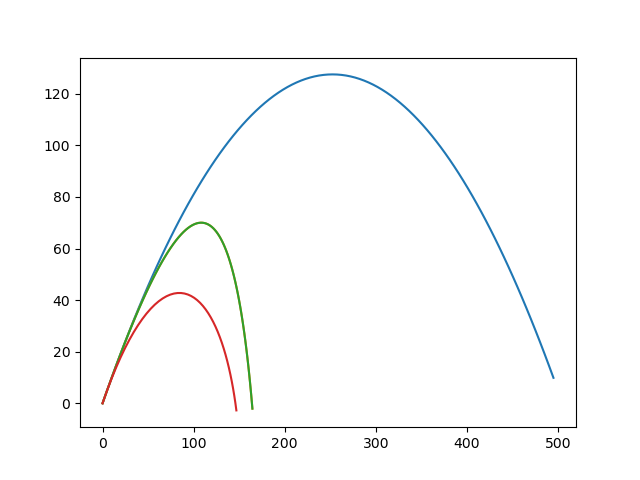
\includegraphics[width=.5\textwidth]{golfPlotTheta45.0.png}
Made with command "make golf THETA=45"

\section*{Contributions}

All work presented is my own. Collaboration with teammates was done minimally and buy and large for "sanity checks". Differential equation solutions were compared, but no code or figures were.


\end{document}

